\documentclass[12pt,letterpaper]{article}

\usepackage[utf8]{inputenc}
\usepackage[T1]{fontenc}
\usepackage{amsmath}
\usepackage{amsfonts}
\usepackage{amssymb}
\usepackage{amsthm}
\usepackage[left=2cm,right=2cm,top=2cm,bottom=2cm,headheight=22pt]{geometry}
\usepackage{fancyhdr}
\usepackage{setspace}
\usepackage{lastpage}
\usepackage{graphicx}
\usepackage{caption}
\usepackage{subcaption}
\usepackage{paralist}
\usepackage{url}

\theoremstyle{definition}
\newtheorem{question}{Question}
\newtheorem{example}{Example}
\newtheorem{exercise}[question]{Exercise}
\newtheorem*{challenge}{Challenge}
\newtheorem*{theorem}{Theorem}
\newtheorem*{definition}{Definition}

\begin{document}

%Paramètres de mise en forme des paragraphes selon les normes françaises
\setlength{\parskip}{1ex plus 0.5ex minus 0.2ex}
\setlength{\parindent}{0pt}

%Paramètres relatifs aux en-têtes et pieds de page.
\pagestyle{fancy}
\lhead{Theron J Hitchman}
\chead{\Large Reading and Guided Practice \#3}
\rhead{Fall 2013}
\lfoot{\emph{Math and Decision Making}}
\cfoot{}
\rfoot{\emph{\thepage\ of \pageref{LastPage}}}

\section*{Introduction}
We introduce more techniques for computing probabilities, and meet the important concept of \emph{independence}.

\section*{Goals}
At the end of this assignment, a student should be able to:
\begin{compactitem}
\item Compute probabilitites of compound events.
\item Recognize and reinterpret some events as compound events.
\item Describe what is meant by independence of two events.
\item Use the multiplication rule for computing probabilities of compound events.
\item Use decision trees to compute probabilities.
\end{compactitem}
A student might also be able to:
\begin{compactitem}
\item Come up with a description for the use of the word ``and'' in compound events as a thing having to do with sets.
\end{compactitem}

\section*{Reading and Questions for 16 November}

\subsection*{Compound Events} %introduce compound events, give laplace-, observe multiplication rule.

In some games of chance, or other situations where probabilities are important, things are arranged so there is a sequence of random events happening, but the bet is only on the final outcome. 
This is a situation where one has a \emph{compound event}: more than one thing must happen in a sequence during any particular trial.

\begin{example}[A Compound Event]
Consider a situation where we have an urn  with some colored balls inside: two red balls and one green ball.
A trial consists of the following:
\begin{compactitem}
\item choose a ball and note its color,
\item replace the ball in the urn and mix the balls around, and 
\item choose a new ball from the urn and note its color.
\end{compactitem}
This kind of situation is often called a \emph{choice with replacement} because we put the chosen item back in before we make the next choice.

This is a compound event because we make a sequence of two choices. 
What is the probability of getting two red balls?

The analysis of this set up can be a little tricky.
In my view, the clearest description comes from remembering that each of the three balls is equally likely at each stage.
There is a perceived imbalance (or bias) toward red because there are more red balls.
To simplify things, we will label the balls as follows: $R1$, $R2$, and $G$ for red-one, red-two, and green.
Now our sample space can be set out as the elements of this table:
\begin{center}
\begin{tabular}{c c c}
R1, R1 & R1, R2 & R1, G \\
R2, R1 & R2, R2 & R2, G \\
G, R1 & G, R2 & G, G 
\end{tabular}
\end{center}
Now each of these nine outcomes is equally likely.
The event of choosing two red balls is the set of four outcomes in the upper left corner.
We deduce that the probability of two red balls in a row here is $4/9$.
\end{example}

Another way to look at this is to realize this as two different choices. 
In the first choice, we have a $2/3$ probability of choosing a red ball. 
In the second choice we also have a $2/3$ probability of choosing a red ball.
It looks like we can just multiply: $2/3 \times 2/3 = 4/9$.
Hey, that is a nifty rule!

But take care.
Multiplication won't always work in set-ups of compound events.

\subsection*{Limits of the multiplication rule} % go to full laplace, introduce independence, state multiplication rule clearly.

Let us reconsider Laplace's Challenge from our first reading about probability.

\begin{quotation}
You have two urns.
Urn 1 (labeled ``heads'') has 3 red balls in it and 1 green ball in it.
Urn 2 (labeled ``tails'') has 1 red ball in it and 3 green balls in it.
The experiment to be conducted is to flip a coin, and then choose two balls from the corresponding urn, \emph{with replacement}. 
What is the probability of drawing two red balls in a row?
\end{quotation}

This set-up is different.
First, there are three stages: filp a coin, choose a ball, then choose a ball.
Second, and more importantly, the two urns are different, so the chances of choosing a red ball \emph{depends upon the outcome of the coin flip}!

This requires some serious reconsideration.
The concept here is that of when two events are ``entangled'' or not.
We have a useful word for keeping these situations apart:

\begin{definition} Two events are called \emph{independent} if the set of possible outcomes of each is unaffected by the outcomes of the other.
\end{definition}

Our first choice with replacement example had two independent events.
The outcome of the first choice of a ball had no effect on the second ball, and, of course, the second ball couldn't affect the first.

But Laplace's Challenge is different.
The choices made in step two and three depend quite clearly on the outcome of the coin flip.
The events here are \underline{not} independent.

Let us state the rule for multiplication clearly:
\begin{quotation}
If two events $A$ and $B$ are independent, then the probability of getting $A$ on the first choice and $B$ on the second (or vice versa), is
\[
\mathrm{Pr}(\text{$A$ and $B$}) = \mathrm{Pr}(A) \times \mathrm{Pr}(B)
\]
\end{quotation}


\subsection*{A Solution to Laplace's Challenge} %introduce and use a decision tree

Another way to organize things here is in a \emph{decision tree}.
We make a diagram of the outcomes possible and note the probabilities of the choices along the way.
The diagram itself is better explanation than any paragraph.
Because it will get hard to read, I'll just draw out the diagram for the first two stages here, and only start the third and final level.

\begin{figure}[h]
\centering
    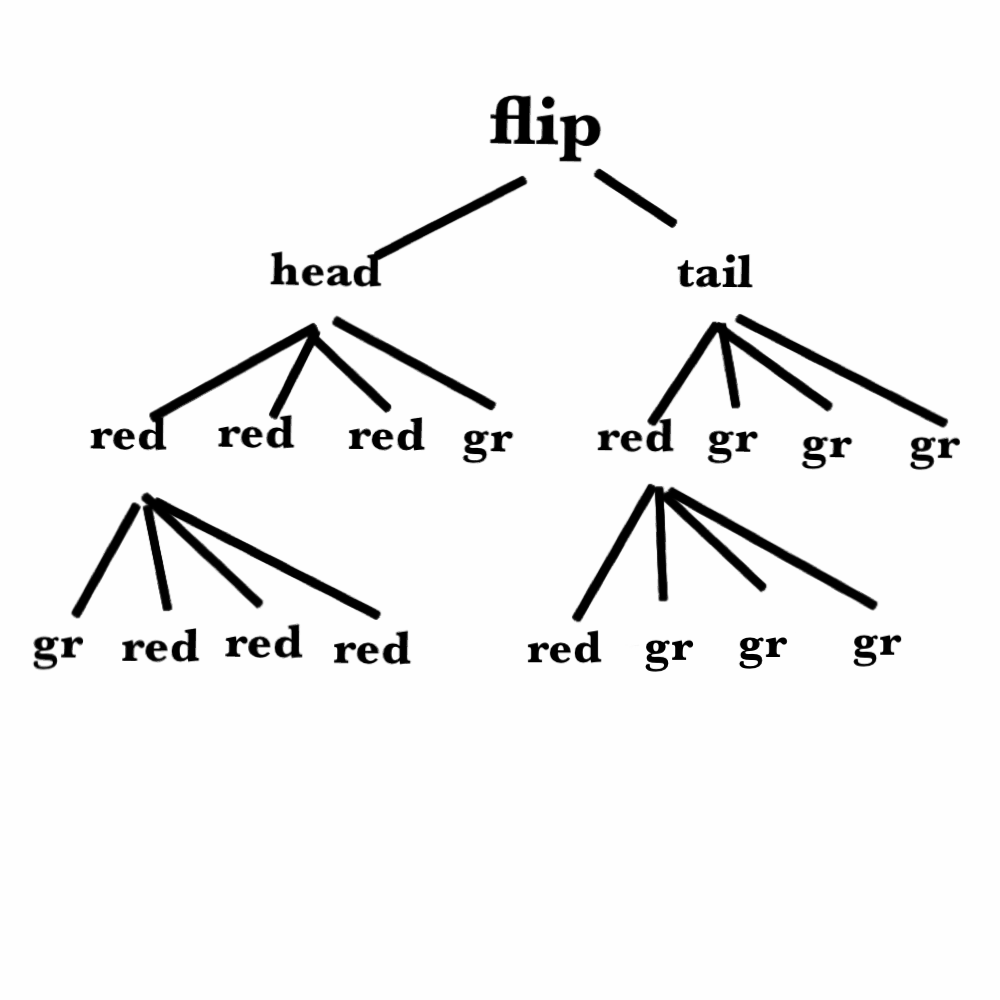
\includegraphics[width=.5\textwidth]{dec-tree.png}
\end{figure}

Note that under each choice we get one branch for each possible outcome of that choice.
At each stage those possible outcomes are all equally likely.

\begin{exercise}
Complete the decision tree diagram by the third row showing the outcomes of the final choice. 
You might have to get a fresh piece of paper and use space more wisely.

At the end you should have 32 ends.
These ends are all of the outcomes in our sample space.
Count the number of ends that correspond to two red balls in a row, and use this to compute the probability of getting two balls in a row in Laplace's challenge.
\end{exercise}

\subsubsection*{Some Practice: Choosing Two cards}

Now you have a bunch of tools to work with.
Use decision trees, the concept of independence and the multiplication rule to answer the following questions.


\begin{exercise}
Consider a random event which consists of drawing two cards from a standard pack of playing cards. What are the probabilities of drawing:
\begin{compactdesc}
\item[(a)] Two hearts in a row, if the draw is made with replacement?
\item[(b)] Two hearts in a row, if the draw is made without replacement?
\item[(c)] Two cards neither of which is a heart, if the draw is made with replacement?
\item[(d)] Two cards neither of which is a heart, if the draw is made without replacement?
\end{compactdesc}
\end{exercise}

You should find that the probabilities are: (a) $1/16$; (b) $1/17$ ; (c) $9/16$ ; and (d) $19/34$. I've simplified them to as not to give away exactly how those numbers come up.


\subsection*{Compound events and the word ``and''} % do the two examples of drawing a single card

Note that our muliplication rule uses the word ``and.''
This can be stretched to cover other situation, where it might not be so obvious that we are dealing with a compound event.
Here are two examples of situations where the word ``and'' is used, either implicitly or explicitly, and the analysis can be handled like a compound event as a result.

\begin{example}
Choose one card from a regular deck of 52 playing cards.
What is the probability that the card is a red queen?

We must find a card which is red \textbf{and} is a queen. 
This is combining two events.
Those things are independent events. 
(Check it!)
So by the multiplication rule: $\mathrm{Pr}(\text{red queen}) = \mathrm{Pr}(\text{red}) \times \mathrm{Pr}(\text{queen}) = 26/52 \times 4/52 = 1/26$.
\end{example}

\begin{example}
Choose one card from a regular deck of 52 playing cards.
What is the probability that the card is red and not a spade?

The two events here are: ``The card is red.'' and ``The card is not a spade.''
These two events are \emph{not} indepdent. 
(Check it!)
So the multiplication rule does not work.
To see this, note:  $\mathrm{Pr}(\text{red}) = 26/52$ and $\mathrm{Pr}(\text{not a spade}) = 39/52$.
But $\mathrm{Pr}(\text{red and not a spade}) = 26/52$.
\end{example}

\begin{exercise}
Describe the sample space and use your description to check the work in the last two examples.
\end{exercise}

\subsection*{A Challenge} % what is and in terms of sets?

\begin{challenge}
We saw that when we think of events as subsets of the sample space, the word ``or'' ends up corresponding to a construction on sets called the ``union.''
What does the word ``and'' correspond to? 
Describe the situation as clearly as you can.
\end{challenge}



%\begin{thebibliography}{9}
%\end{thebibliography}

\end{document}
%sagemathcloud={"zoom_width":100}